\documentclass[12pt]{article}
\usepackage{scrextend}
\usepackage[utf8]{inputenc}
\usepackage[polish]{babel}
\usepackage[T1]{fontenc}%polskie znaki
\usepackage[utf8]{inputenc}%polskie znaki
\usepackage{geometry}
\usepackage{float}
\usepackage{enumitem}
\usepackage{hyperref}
\usepackage{graphicx}
\usepackage{amsmath}

\renewcommand{\baselinestretch}{1.5}


\begin{document}

\begin{flushleft}
    Damian Koper \textbf{241292} \\
\end{flushleft}
\vspace{1cm}
{
    \centering
    {\Huge\scshape\bfseries Modelowanie i analiza systemów informatycznych }\\
    \large{Sieci Petriego - konstrukcja sieci Petriego z łukami hamującymi (cz. 2)}\\
    \vspace{0.5cm}
}
\newcounter{ex}
\setcounter{ex}{0}
\newcommand{\ex}[1]{
    \refstepcounter{ex}{
        \noindent\normalfont\Large\bfseries Zadanie \arabic{ex}.
    } \\
    #1
}
\clearpage
\ex{Rozbudowa sieci - tramwaje}
\vspace{-0.5cm}

\begin{figure}[H]
    \centering
    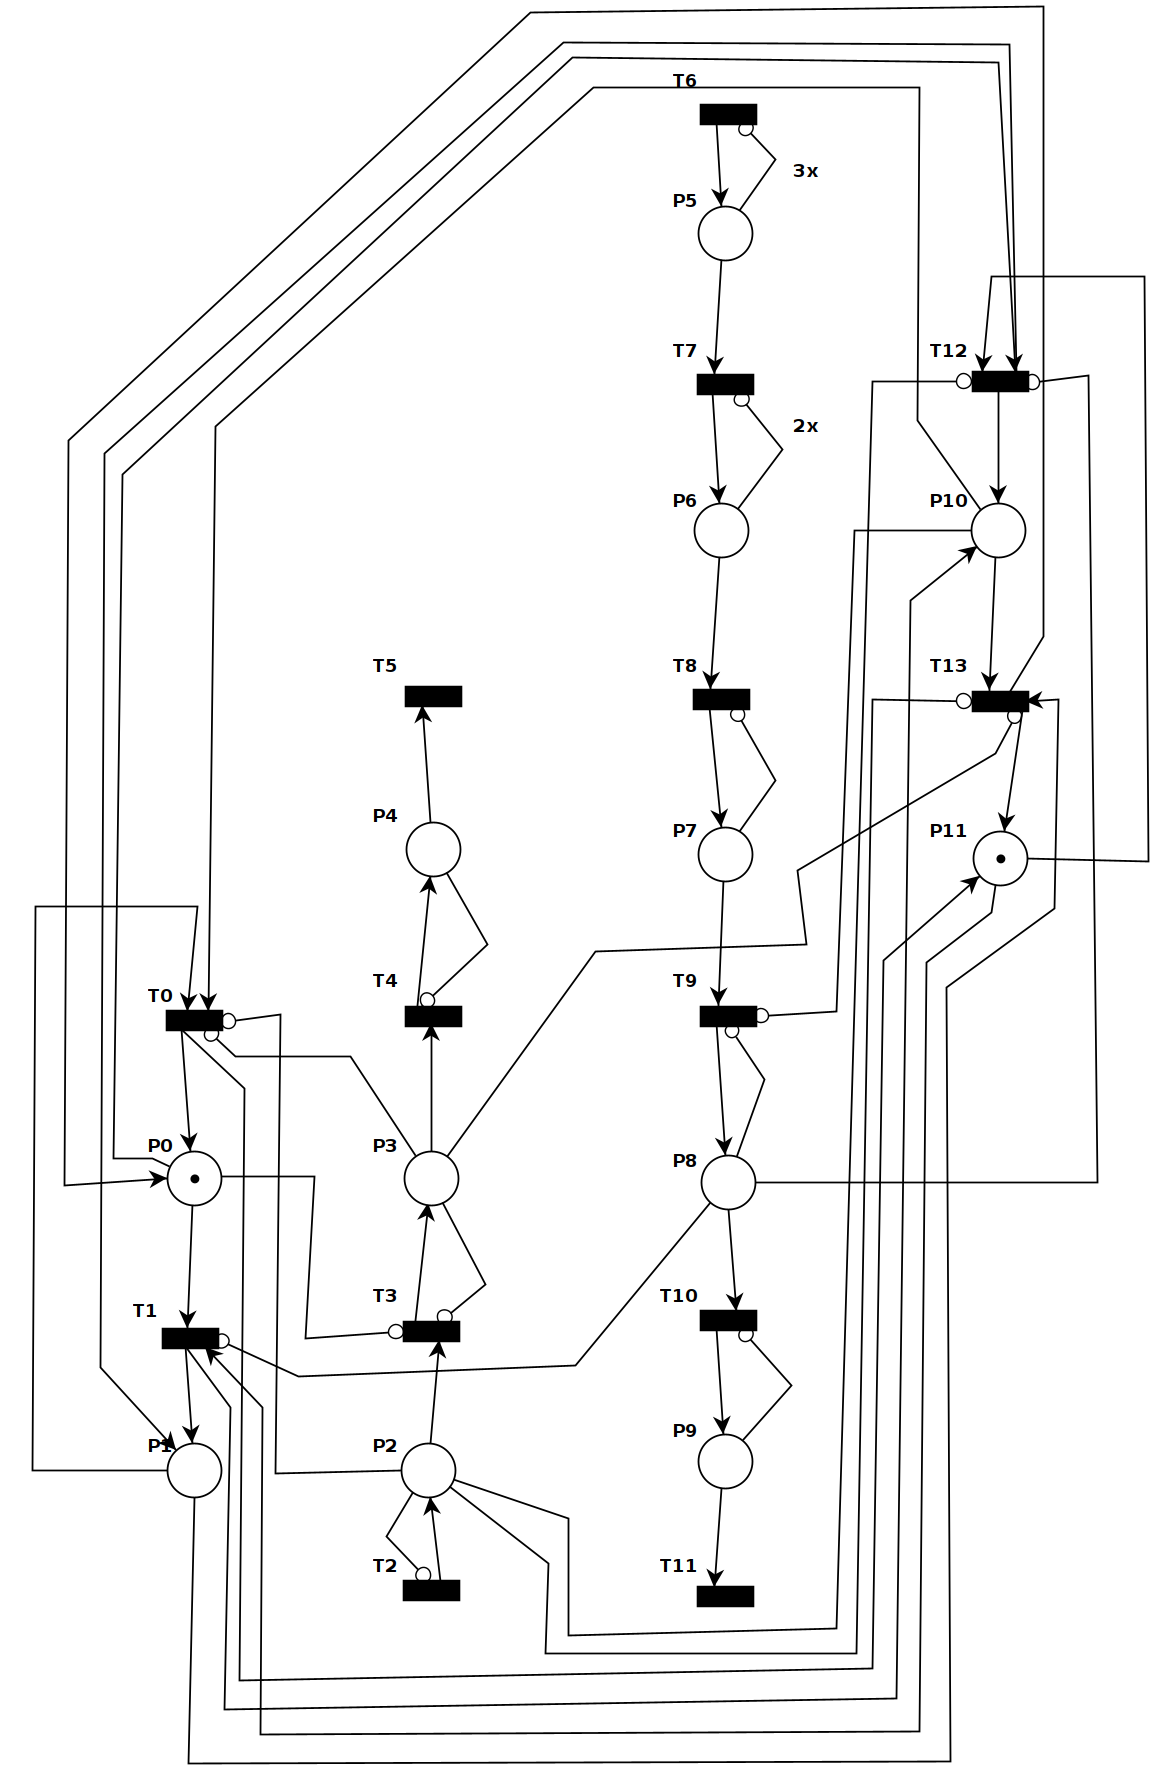
\includegraphics[width=0.7\linewidth]{../../lab8/ex_1}
    \caption{Semafory naprzemienne. Nie można przełączyć automatycznie z $p_{11}$ na $p_{10}$ semafora prawego, kiedy w $p_{2}$ pojawi się tramwaj.}
\end{figure}

\clearpage

\ex{Redukcja sieci}
\vspace{-0.5cm}

\begin{figure}[H]
    \centering
    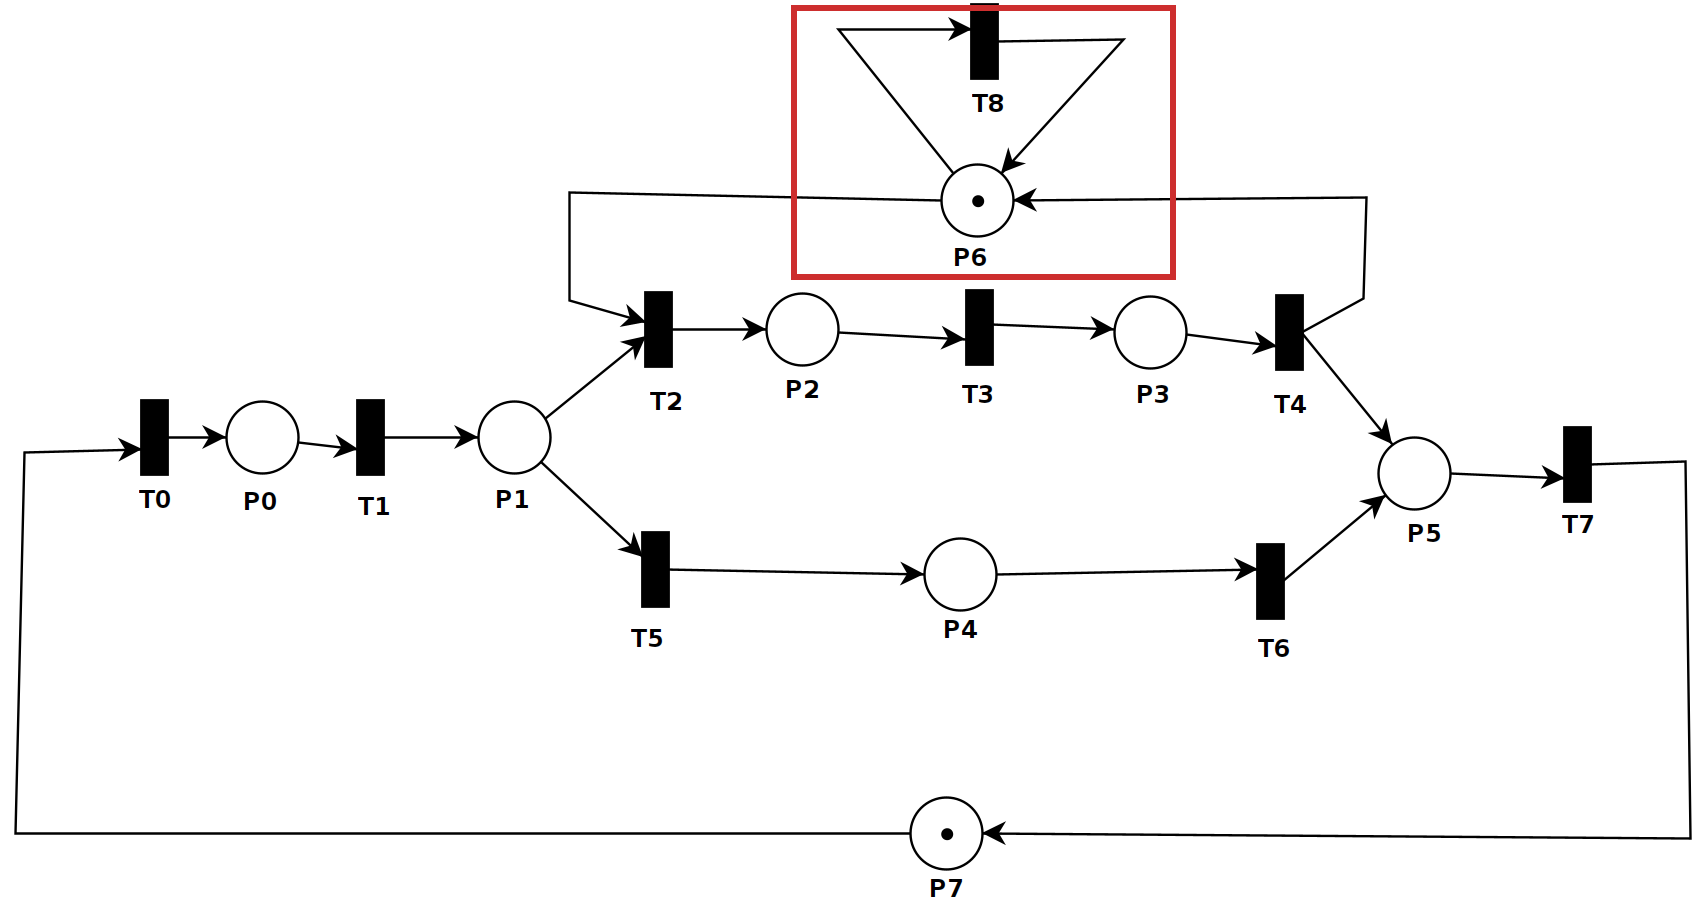
\includegraphics[width=\linewidth]{../../lab8/ex_2_1}
    \caption{Sieć przed redukcją. Redukcja F.}
\end{figure}

\begin{figure}[H]
    \centering
    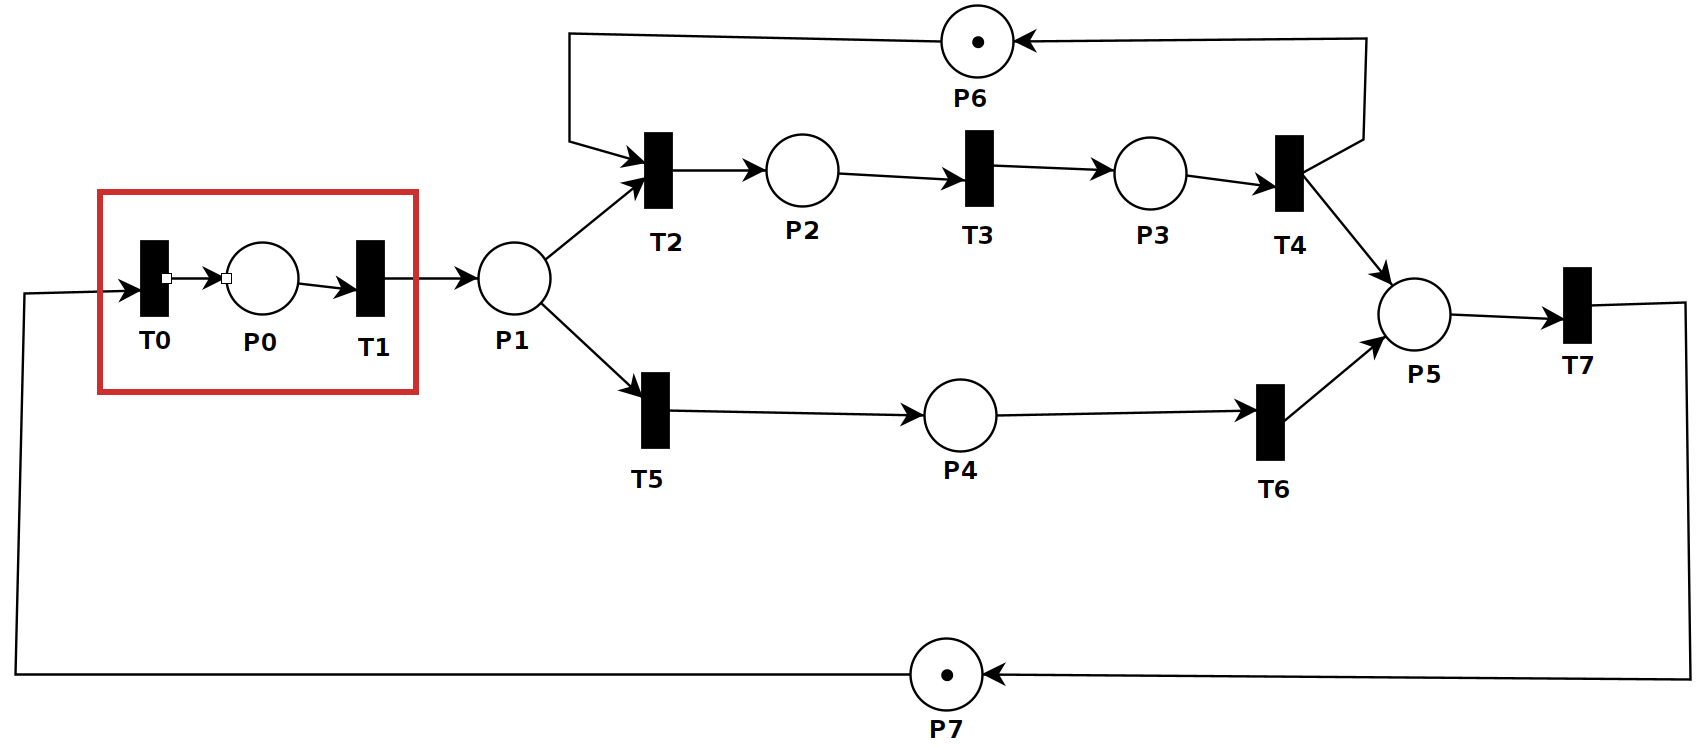
\includegraphics[width=\linewidth]{../../lab8/ex_2_2}
    \caption{Sieć po redukcji. Redukcja B.}
\end{figure}

\begin{figure}[H]
    \centering
    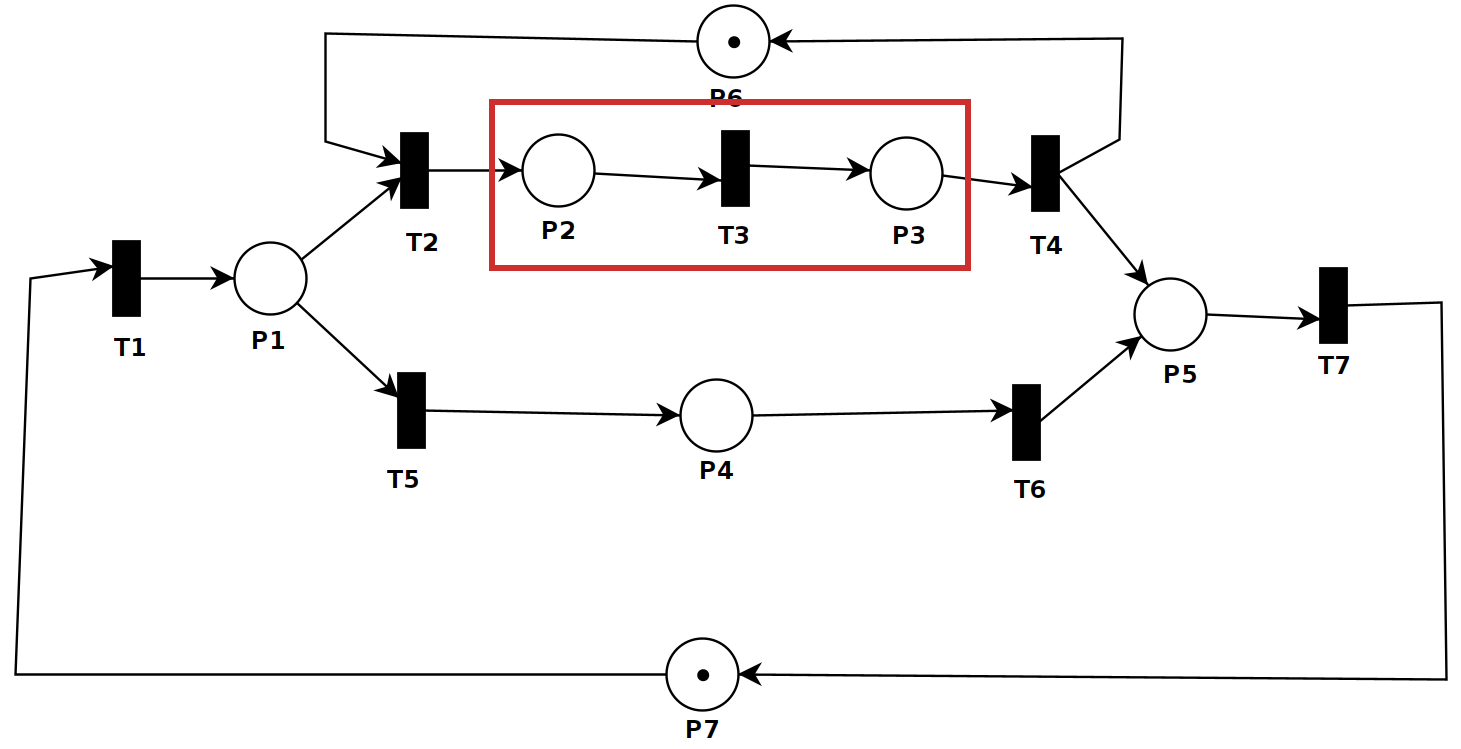
\includegraphics[width=\linewidth]{../../lab8/ex_2_3}
    \caption{Sieć po redukcji. Redukcja A.}
\end{figure}

\begin{figure}[H]
    \centering
    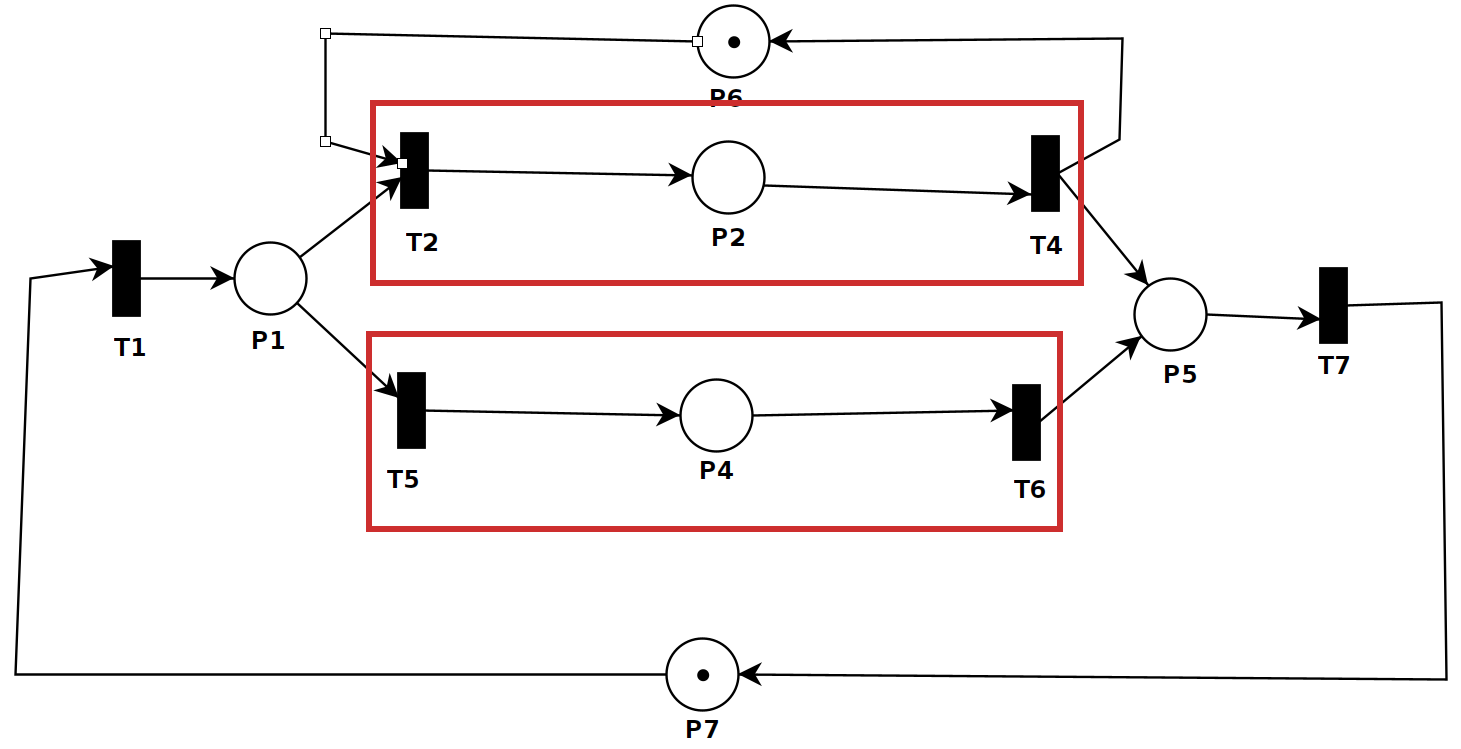
\includegraphics[width=\linewidth]{../../lab8/ex_2_4}
    \caption{Sieć po redukcji. Redukcja B.}
\end{figure}

\begin{figure}[H]
    \centering
    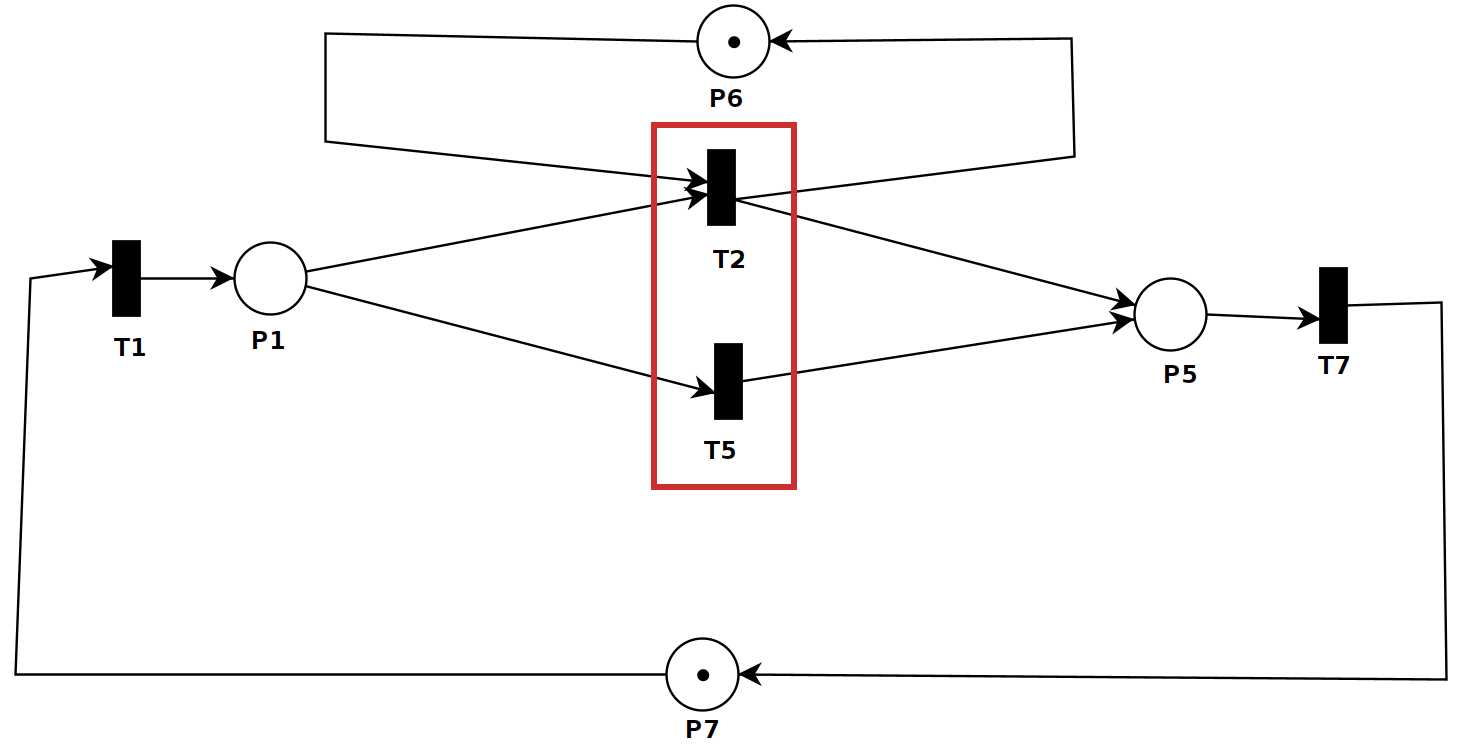
\includegraphics[width=\linewidth]{../../lab8/ex_2_5}
    \caption{Sieć po redukcji. Redukcja D.}
\end{figure}

\begin{figure}[H]
    \centering
    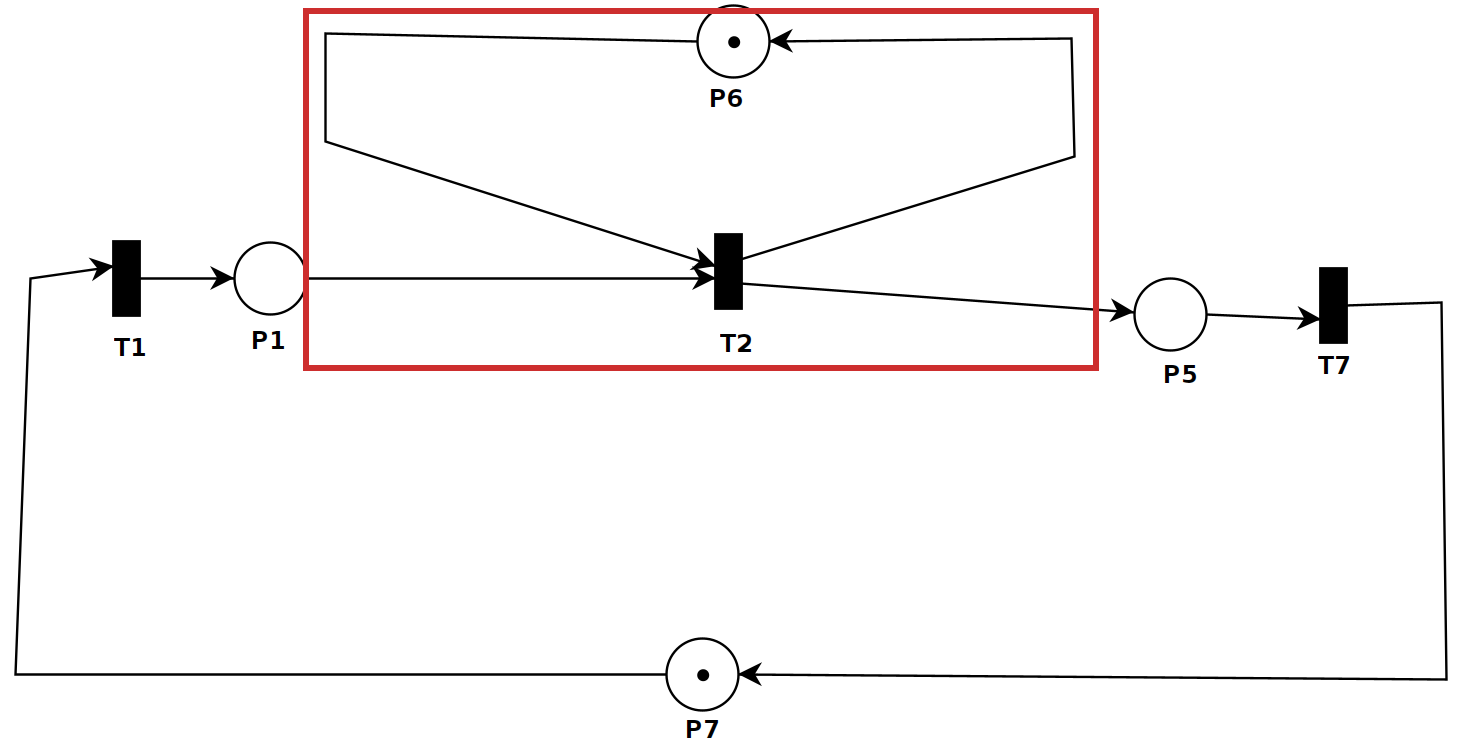
\includegraphics[width=\linewidth]{../../lab8/ex_2_6}
    \caption{Sieć po redukcji. Redukcja E.}
\end{figure}

\begin{figure}[H]
    \centering
    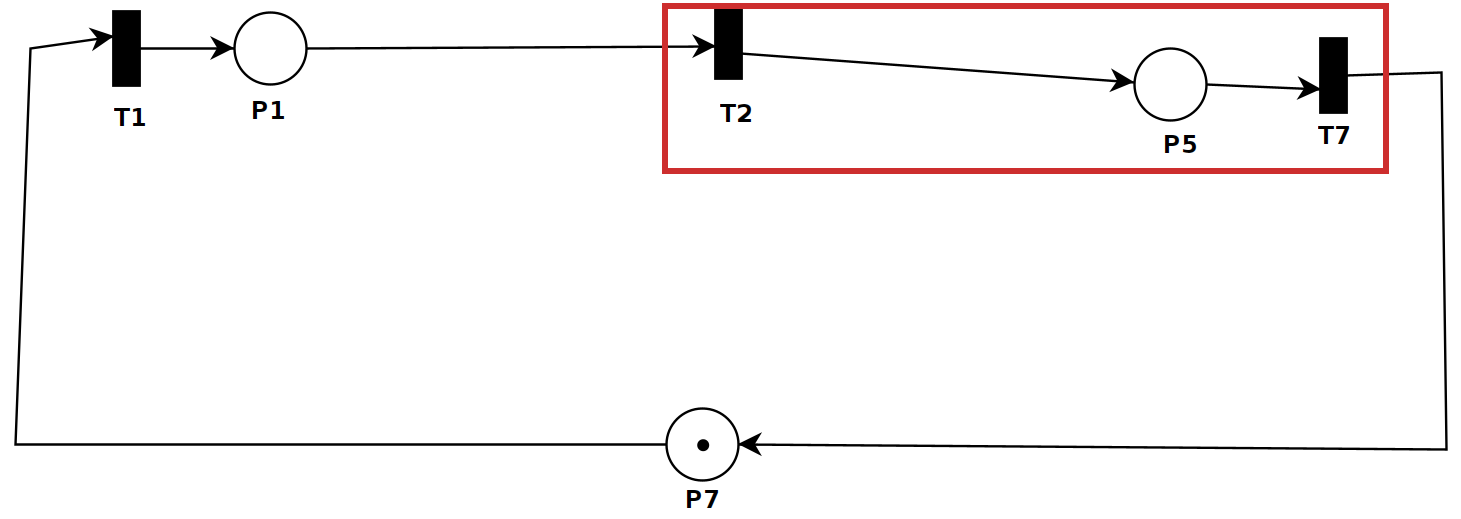
\includegraphics[width=\linewidth]{../../lab8/ex_2_7}
    \caption{Sieć po redukcji. Redukcja B.}
\end{figure}


\begin{figure}[H]
    \centering
    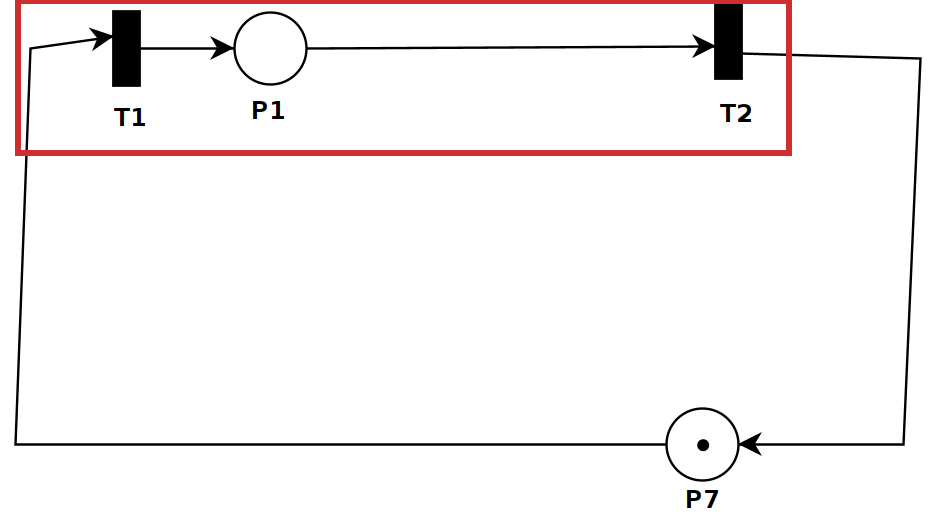
\includegraphics[width=\linewidth]{../../lab8/ex_2_8}
    \caption{Sieć po redukcji. Redukcja B.}
\end{figure}

\begin{figure}[H]
    \centering
    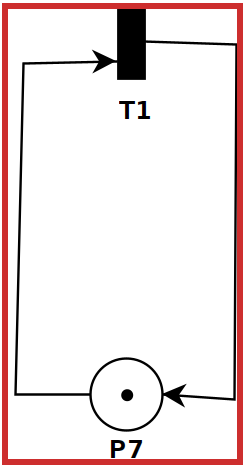
\includegraphics[width=0.2\linewidth]{../../lab8/ex_2_9}
    \caption{Sieć po redukcji. Redukcja F.}
\end{figure}

\begin{figure}[H]
    \centering
    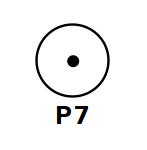
\includegraphics[width=0.2\linewidth]{../../lab8/ex_2_10}
    \caption{Sieć po redukcji.}
\end{figure}
\end{document}